% chap3.tex
%

\newif\ifcompress
\compresstrue   % Uncomment this line for the authors
\compressfalse % Uncomment these two lines for anonymous review

\mychapter{Joint reasoning over text and KB for answer generation}

%Previous work has largely ignored a key problem in question recommendation, i.e., whether the potential answerer is likely to accept and answer the recommended questions in a timely manner. 

\noindent 
In this work I propose to enrich the input data representation for QA systems by combining available unstructured, semi-structured and structured data sources for joint reasoning, which can improve the performance of question answering over both text collections and knowledge bases.


\section{Joint reasoning over text and KB for answer generation}


\subsection{Text-based QA}

\begin{figure}
\centering
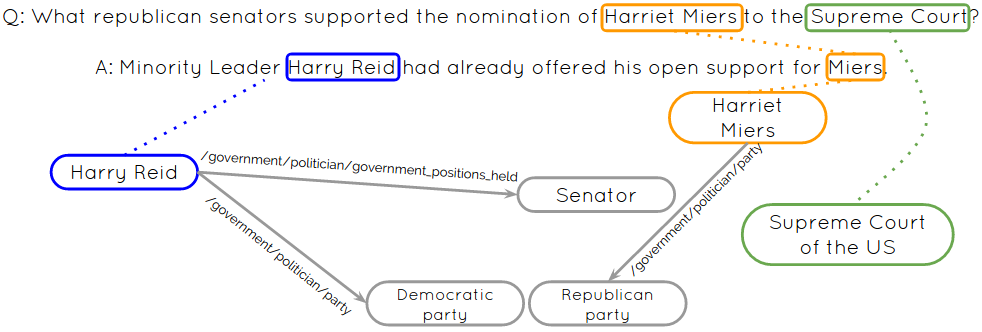
\includegraphics[width=1.0\textwidth]{figures/text_kb}
\caption{Annotation of natural language text with mentioned entities and their subgraphs in a knowledge base}
\label{fig:text_kb}
\end{figure}

For question answering over text corpora I propose to extend the text representation with annotations about mentioned entities and their relations from open \cite{Fader:2014:OQA:2623330.2623677} or schema-based knowledge bases (e.g. dbPedia or Freebase).
Such representation allows not only find different mentions of the same entity, but also look into the connections of the mentioned entities in order to learn more about the candidate answer.
For example, for the question mentioned in the introduction \textit{``What republican senators supported the nomination of Harriet Miers to the Supreme Court?''} and a candidate answer sentence \textit{``Minority Leader Harry Reid had already offered his open support for Miers.''}, such joint text-KB representation can look like Figure \ref{fig:text_kb}.
A QA system can discover that ``Harry Reid'' political affiliation is with the Democratic Party, and he cannot be referred to as ``republican senator''.
In other cases using a KB as an additional source of information may reveal specific connections between entities in the question and in the answer candidates.
For example, for another TREC QA 2007 question \textit{``For which newspaper does Krugman write?''} and retrieved candidate answer \textit{New York Times} a path between ``Paul Krugman'' and ``New York Times'' in the knowledge graph gives an evidence in support of the candidate.

More specifically, to do this kind of inference I propose:
\begin{itemize}
\item use existing approaches for document retrieval (e.g. web search using question as a query \cite{tsai2015web}) and candidate answer extraction.
\item perform entity linking to mentions of KB entities in questions and corresponding candidate answers.
\item for each mentioned entity extract a subgraph containing its neighborhood up to certain number of edges away and paths to other mentioned entities.
\item follow machine learning approach for candidate answer ranking and extend the feature representation with features derived from subgraph analysis. Examples of features are:
	\begin{itemize}
	\item features describing discovered connections between entities mentioned in a question and a candidate answer, such as indicators of the relations, combination of relations with words and n-grams from the questions, similarity between the relations and the question text (using tf-idf or embeddings representation), etc. Textual representations of the predicates in structured knowledge bases can be obtained either from its description or using patterns learned from a large collection using distant supervision \cite{MintzBSJ09}.
	\item features describing the entities mentioned in the answer, i.e. similarities between entity properties and question words, n-grams and phrases, etc.
	\end{itemize}
\end{itemize}

For training text-based QA model I propose to use available QnA pairs from community question answering websites, which represent real user tasks and after certain filtering can be a good fit for training both factoid and non-factoid question answering systems.
The data can help to learn more associations between the language used in questions and their corresponding answers, which can be encoded as conditional probabilities (e.g. $p(w_a|w_{q_1},...,w_{q_n}$, where $w_a$ is a word of the answer and $w_{q_i}$ is some subset of the question words), pointwise mutual information or by employing deep learning techniques \cite{WangN15}.

\subsection{Knowledge base QA}

\begin{figure}
\centering
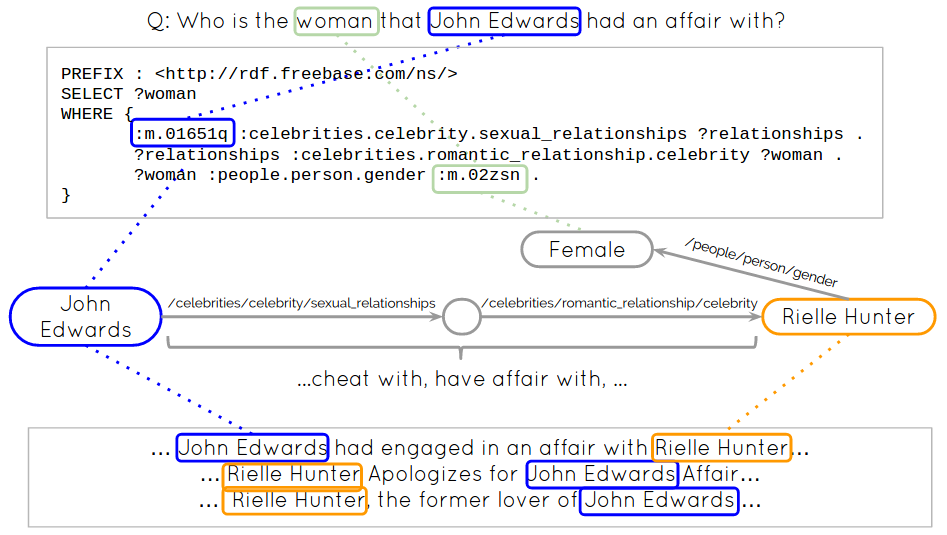
\includegraphics[width=1.0\textwidth]{figures/kb_text}
\caption{Annotation of KB graph nodes and edges with unstructured text data}
\label{fig:kb_text}
\end{figure}

\begin{table}
\centering
\caption{Example of a question from WebQuestions dataset with related unstructured information}
\begin{tabular}{| p{5cm} | p{11cm} |} \hline
Question & Who is the woman that John Edwards had an affair with?\\
\hline
Provided answer & ``Writer'', ``Politician'', ``Lawyer'', ``Attorneys in the United States''\\
\hline
Correct answer & Rielle Hunter\\
\hline
Phrase from Wikipedia & John Edwards had engaged in an affair with Rielle Hunter...\\
\hline
QnA pair from Yahoo! Answers & Who was it that John Edwards had an affair with? Today, John Edwards admitted to having an affair with filmmaker Rielle Hunter.\\
\hline
\end{tabular}
\label{table:kbqa_example}
\end{table}

Lexicons learned during training of a knowledge base question answering systems are limited and often needs to be retrained to include additional data.
To complement the lexicon learned during training for candidate structured query scoring I propose to use unstructured text data related to mentioned entities and predicates (see Figure \ref{fig:kb_text}).
For example, Table \ref{table:kbqa_example} shows an example of a question from the WebQuestions dataset, that is answered incorrectly by a state-of-the-art system.
A similar question is missing from the training set, however, an easy web search can retrieve a relevant sentence, which give enough supporting evidence to answer this question correctly.

More specifically, I propose:
\begin{itemize}
\item Use one of the available state of the art systems, such as \cite{bastmore:cikm:2015:aquu}, as a baseline.
\item Extend a set of features representing a candidate answer with features derived from unstructured text fragments:
	\begin{itemize}
	\item from large document collection (such as the web) retrieve a set of passages by querying a search system with question, question + answer, question and answer entities as queries.
	\item find mentions of answer entities in the passages and use some aggregated statistics as features for the corresponding candidates.
	\item for each candidate answer retrieve a set of patterns used to express the corresponding predicates obtained using distant supervision from a large text collection and compute the similarities between these patterns and the question text.
	\end{itemize}
\end{itemize}

In addition, similar to text-based systems, I propose to include QnA pairs from CQA websites as weakly labeled training data.
For example, a question similar to the one presented in Table \ref{table:kbqa_example} is not present in the labeled training set, but can easily be found in Yahoo! Answers\footnote{http://answers.yahoo.com/}.
CQA data should be preprocessed (possibly filtered by categories of the questions and other heuristics), and select QnA pairs mentioning at least one entity in the question and in the answer.
After a reasonable cleanup such QnA pairs can be used for training treating answer entities as the correct answer.

% Finally, to solve the problem of compositionality of queries following the idea proposed in \cite{ReddyLS14} learn lexical features from raw sentences and their distantly supervised alignments to a KB, but avoid expensive and innaccurate semantic parsing step and learn direct associations between surface features and KB elements.
% \textbf{Actually I don't have a very good idea how to do this, probably need to remove this paragraph}.

\section{Summary}

